%!TEX root = ../Report.tex
\chapter{OCamlFUSE}
\label{chp:analysis}
OCamlFUSE is a FUSE file system implementation written by Alessandro Strada to mount a Google Drive directory onto the Linux file system. It provides capabilities for reading from and writing to files and folders, accessing documents saved in Google product formats, handling duplicate files, and many other remote file system operations. \cite{gdriveocamlfuse}
\section{Explore OCamlFUSE Source Code}
\subsection{Summary}
  \begin{enumerate}
  \item Source code downloaded from GitHub. \cite{gdriveocamlfuse}
  \item ML versus MLI file. The first thing I noticed was that there were duplicate files in the source folder that simply had
    different extensions. After some research, I found that the
    extension ML stands for Meta Language which is the umbrella
    programming language that contains OCaml. I suspect that the
    extension MLI stands for Meta Language Interface, but I cannot be
    certain of that since I was unable to find its expansion in my
    research. The reason I suspect it is Interface is because of what
    I observed when I looked at the files themselves.  I opened
    bufferPool.ml and bufferPool.mli and compared them to each
    other. In the ML file, I found full function implementations while
    in the MLI file, I found a listing of function signatures. So, the
    MLI files must be interfaces that are used by other classes so as
    to hide the implementation in the ML from users. Dr. Mateti clarified for me that MLI files are compiled from ML files.
  \item SLOCCOUNT
  \begin{verbatim}
hanen@hanen:~$ sloccount /home/hanen/Desktop/google-drive-
ocamlfuse-beta/
Have a non-directory at the top, so creating directory top_dir
Adding /home/hanen/Desktop/google-drive-ocamlfuse-beta//LICENSE
to top_dir
Adding /home/hanen/Desktop/google-drive-ocamlfuse-beta//Makefile
to top_dir
Adding /home/hanen/Desktop/google-drive-ocamlfuse-beta//README.md
to top_dir
Adding /home/hanen/Desktop/google-drive-ocamlfuse-beta//_config.yml
to top_dir
Creating filelist for bin
Creating filelist for doc
Adding /home/hanen/Desktop/google-drive-ocamlfuse-beta//dune-project
to top_dir
Adding /home/hanen/Desktop/google-drive-ocamlfuse-beta//google-
drive-ocamlfuse.opam to top_dir
Creating filelist for test
Creating filelist for tools
Have a non-directory at the top, so creating directory src_top_dir
Adding /home/hanen/Desktop/google-drive-ocamlfuse-beta//src/
appDir.ml
to src_top_dir
Adding /home/hanen/Desktop/google-drive-ocamlfuse-beta//src/
bufferPool.ml
to src_top_dir
Adding /home/hanen/Desktop/google-drive-ocamlfuse-beta//src/
bufferPool.mli
to src_top_dir
Adding /home/hanen/Desktop/google-drive-ocamlfuse-beta//src/
buffering.ml
to src_top_dir
Adding /home/hanen/Desktop/google-drive-ocamlfuse-beta//src/
buffering.mli
to src_top_dir
Adding /home/hanen/Desktop/google-drive-ocamlfuse-beta//src/
cache.ml
to src_top_dir
Adding /home/hanen/Desktop/google-drive-ocamlfuse-beta//src/
cache.mli
to src_top_dir
Adding /home/hanen/Desktop/google-drive-ocamlfuse-beta//src/
cacheData.ml
to src_top_dir
Adding /home/hanen/Desktop/google-drive-ocamlfuse-beta//src/
cacheData.mli
to src_top_dir
Adding /home/hanen/Desktop/google-drive-ocamlfuse-beta//src/
concurrentGlobal.ml
to src_top_dir
Adding /home/hanen/Desktop/google-drive-ocamlfuse-beta//src/
config.ml
to src_top_dir
Adding /home/hanen/Desktop/google-drive-ocamlfuse-beta//src/
context.ml
to src_top_dir
Adding /home/hanen/Desktop/google-drive-ocamlfuse-beta//src/
dbCache.ml
to src_top_dir
Adding /home/hanen/Desktop/google-drive-ocamlfuse-beta//src/
dbCache.mli
to src_top_dir
Adding /home/hanen/Desktop/google-drive-ocamlfuse-beta//src/
drive.ml
to src_top_dir
Adding /home/hanen/Desktop/google-drive-ocamlfuse-beta//src/dune
to src_top_dir
Adding /home/hanen/Desktop/google-drive-ocamlfuse-beta//src/
gaeProxy.ml
to src_top_dir
Adding /home/hanen/Desktop/google-drive-ocamlfuse-beta//src/
keyValueStore.ml
to src_top_dir
Adding /home/hanen/Desktop/google-drive-ocamlfuse-beta//src/
memoryCache.ml
to src_top_dir
Adding /home/hanen/Desktop/google-drive-ocamlfuse-beta//src/
memoryCache.mli
to src_top_dir
Adding /home/hanen/Desktop/google-drive-ocamlfuse-beta//src/
mime.ml
to src_top_dir
Adding /home/hanen/Desktop/google-drive-ocamlfuse-beta//src/
oauth2.ml
to src_top_dir
Adding /home/hanen/Desktop/google-drive-ocamlfuse-beta//src/
state.ml
to src_top_dir
Adding /home/hanen/Desktop/google-drive-ocamlfuse-beta//src/
threadPool.ml
to src_top_dir
Adding /home/hanen/Desktop/google-drive-ocamlfuse-beta//src/
threadPool.mli
to src_top_dir
Adding /home/hanen/Desktop/google-drive-ocamlfuse-beta//src/
utils.ml
to src_top_dir
Categorizing files.
Finding a working MD5 command....
Found a working MD5 command.
Computing results.

SLOC    Directory       SLOC-by-Language (Sorted)
7834    src_top_dir     ml=7834
663     bin             ml=663
211     test            ml=211
76      tools           sh=76
0       doc             (none)
0       top_dir         (none)

Totals grouped by language (dominant language first):
ml:            8708 (99.13%)
sh:              76 (0.87%)

Total Physical Source Lines of Code (SLOC)                = 8,784
Development Effort Estimate, Person-Years (Person-Months) = 1.96 
(23.50)
 (Basic COCOMO model, Person-Months = 2.4 * (KSLOC**1.05))
Schedule Estimate, Years (Months)                         = 0.69 
(8.30)
 (Basic COCOMO model, Months = 2.5 * (person-months**0.38))
Estimated Average Number of Developers (Effort/Schedule)  = 2.83
Total Estimated Cost to Develop                           = 
$ 264,557
 (average salary = $56,286/year, overhead = 2.40).
SLOCCount, Copyright (C) 2001-2004 David A. Wheeler
SLOCCount is Open Source Software/Free Software, licensed under 
the GNU GPL.
SLOCCount comes with ABSOLUTELY NO WARRANTY, and you are welcome 
to redistribute it under certain conditions as specified by the 
GNU GPL license;
see the documentation for details.
Please credit this data as "generated using David A. Wheeler's 
'SLOCCount'."
  \end{verbatim}
  \item Quick Code Exploration
    \begin{enumerate}
    \item There is a Make module in the concurrentGlobal file. 
    \item The file drive.ml appears to have the bulk of logic behind
      this implementation.
    \item I picked a function from the buffer.mli interface file
      called \verb|write_to_block| and did a project wide search for
      it. I found it referenced in the drive.ml file as
      \\ \verb|Buffering.MemoryBuffers.write_to_block|. I do not
      understand why the case is different in the reference. Buffering
      when calling the function versus buffering in the definition of
      the file. I would not have made that connection before, but now
      am aware of it.
    \item Gapi shows up all over the code. It stands for Google API.
    \end{enumerate}
  \end{enumerate}

\subsection{Pseudo-code}
\subsubsection{Class: appDir}
\begin{enumerate}
    \item Getters and Setters
    \begin{enumerate}
        \item \verb|config_path: string|
        \item \verb|data_dir: string|
        \item \verb|cache_dir: string|
        \item \verb|log_dir: string|
        \item \verb|state_path: string|
        \item \verb|app_log_path: string|
        \item \verb|curl_log_path: string|
    \end{enumerate}
    \item \verb|function xdg_data_home| \\
    Try to get the value of the environment variable \verb|XDG_DATA_HOME| and return that value. \\
    If exception thrown trying to get this value, return that it was not found.
    \item \verb|function xdg_config_home| \\
    Try to get the value of the environment variable \verb|XDG_CONFIG_HOME| and return that value. \\
    If exception thrown trying to get this value, return that it was not found.
    \item \verb|function xdg_cache_home| \\
    Try to get the value of the environment variable \verb|XDG_CACHE_HOME| and return that value. \\
    If exception thrown trying to get this value, return that it was not found.
    \item \verb|function get_config_path| \\
    input: \verb|config_path: string, xdg_base_directory: boolean,| \\ \verb|base_dir: string, fs_label: string| \\
    if \verb|config_path| is not empty, then return \verb|config_path| and false (not base directory) \\
    else if \verb|xdg_base_directory| is true, then make directory \verb|xdg_config_dir| and return \verb|xdg_config_path| and true (is base directory) \\
    else if \verb|xdg_config_path| exists, then return \verb|xdg_config_path| and true (is base directory) \\
    else return \verb|default_base_dir| + \verb|fs_label| + "config" if \verb|base_dir| is empty or \verb|base_dir| + \verb|fs_label| + "config"| if \verb|base_dir| is not empty and false (not base directory)
    \item \verb|function create| \\
    input: \verb|config: ConfigFileStore.data, config_path: string,| \\ \verb|base_dir: string, fs_label: string, xdg_base_directory: boolean| \\
    set \verb|data_dir| to \verb|config.Config.data_directory| if \verb|config.Config.data_directory| is not empty \\
    set \verb|data_dir| to \verb|xdg_data_home| + "gdfuse" + \verb|fs_label| if \verb|xdg_base_directory| is true \\
    otherwise, set \verb|data_dir| to \verb|default_base_dir| + \verb|fs_label| if \verb|base_dir| is empty or set \verb|data_dir| to \verb|base_dir| + \verb|fs_label| if \verb|base_dir| is not empty \\
    set \verb|cache_dir| to \verb|config.Config.cache_directory| if \verb|config.Config.cache_directory| is not empty \\
    set \verb|cache_dir| to \verb|xdg_cache_home| + "gdfuse" + \verb|fs_label| if \verb|xdg_base_directory| is true \\
    otherwise, set \verb|cache_dir| to \verb|data_dir| + "cache" \\
    set \verb|log_dir| to \verb|config.Config.log_directory| if \verb|config.Config.log_directory| is not empty \\
    set \verb|log_dir| to \verb|cache_dir| + "log" if \verb|xdg_base_directory| is true \\
    otherwise, set \verb|log_dir| to \verb|data_dir| \\
    set \verb|state_path| to \verb|data_dir| + "state" \\
    set \verb|app_log_path| to \verb|log_dir| + "gdfuse.log" \\
    set \verb|curl_log_path| to \verb|log_dir| + "curl.log" \\
    return \verb|config_path|, \verb|data_dir|, \verb|cache_dir|, \verb|log_dir|
    \item \verb|function create_directories| \\
    input: \verb|app_dir: object| \\
    make directory for \verb|data_dir| from \verb|app_dir| \\
    make directory for \verb|cache_dir| from \verb|app_dir| \\
    make directory for \verb|log_dir| from \verb|app_dir| \\
\end{enumerate}
\subsubsection{Class: buffering}
\textbf{Block: module}
\begin{enumerate}
    \item \verb|function create| \\
    input: \verb|offset: object|, \verb|size: integer|, \verb|mutex: object|, \verb|condition: object|, \verb|buffer_pool: object| \\
    create block and set defaults.
    \item \verb|function blit_to_arr| 
    \item \verb|function blit_from_arr| 
    \item \verb|function flush| \\
    input: \verb|block: object| \\
    if state equals dirty, then 
\end{enumerate}
\textbf{MemoryBuffers: module}
\begin{enumerate}
    \item \verb|function get_block_index| 
    \item \verb|function get_block_start_pos| 
    \item \verb|function remove_block| 
    \item \verb|function remove_full_block| 
    \item \verb|function remove_partial_block| 
    \item \verb|function release_lru_buffer_if_needed| 
    \item \verb|function release_lru_buffer_if_no_free_buffer_left| 
    \item \verb|function release_lru_buffer_if_request_blocked| 
    \item \verb|function flush| 
    \item \verb|function flush_block| 
    \item \verb|function flush_blocks| 
    \item \verb|function flush_lru_buffer_if_needed| 
    \item \verb|function flush_lru_buffer_if_no_free_buffer_left| 
    \item \verb|function flush_lru_buffer_if_request_blocked| 
    \item \verb|function get_block| 
    \item \verb|function read_block| 
    \item \verb|function read_ahead| 
    \item \verb|function remove_buffers| 
    \item \verb|function write_to_block| 
    \item \verb|function evict_cache| \\
    input: \verb|buffers: object| \\
    Loop 10 times and check if the thread needs to be evicted. If it does, then exit.
    Call \verb|flush_lru_buffer_if_request_blocked| and \\ \verb|release_lru_buffer_if_request_blocked|.
    \item \verb|function create_eviction_thread| \\
    input: \verb|buffers: object| \\
    create a thread.
    \item \verb|function stop_eviction_thread| \\
    input: \verb|buffers: object| \\
    set the \verb|stop_eviction_thread| flag to true, so that the thread is exited.
\end{enumerate}
\subsubsection{Class: bufferPool}
\begin{enumerate}
    \item \verb|function create| \\
    input: \verb|pool_size: integer|, \verb|buffer_size: integer| \\
    set \verb|max_buffers| to \verb|pool_size| / \verb|buffer_size| if \verb|pool_size % buffer_size| = 0 \\
    otherwise, set \verb|max_buffers| to \verb|pool_size| / \verb|buffer_size| + 1 \\
    return object containing \verb|max_buffers|, \verb|buffer_count|, \verb|buffer_size|, \verb|free_buffers|, \verb|pending_requests| \\
    \item \verb|function acquire_buffer| \\
    input: \verb|mutex: object|, \verb|condition: object|, \verb|buffer_pool: object| \\
    try to get a free buffer from the Queue. \\
    if the Queue is empty, then: \\
    if \verb|buffer_count| < \verb|max_buffers|, then increase \verb|buffer_count| by 1 and return a new buffer with the buffer's id set to \verb|buffer_count|, mutex set to Mutex.Create(), and condition set to Condition.Create() \\
    else, increase \verb|pending_requests| by 1 and while \verb|free_buffers| is equal to zero, wait. Once, waiting is done, decrease \verb|pending_requests| by 1 and get buffer. \\
    \item \verb|function release_buffer| \\
    input: \verb|buffer: object|, \verb|condition: object|, \verb|buffer_pool: object| \\
    add a buffer to the Queue \\
    wake a thread up
\end{enumerate}
\subsubsection{Class: cache}
\begin{enumerate}
    \item \verb|function create_cache| \\
    create cache with defaults.
    \item \verb|function get_content_path| \\
    input: \verb|cache: object|, \verb|resource: object| \\
    concatenate the cache directory with the remote id.
    \item \verb|function delete_files_from_cache| \\
    input: \verb|cache: object|, \verb|resource: list| \\
    create \verb|remove_file| inline method
    if the file path exists, then remove the file.
    \item \verb|function setup_db| \\
    input: \verb|cache: object| \\
    if in memory, setup cache.
    \item \verb|function clean_up_cache| \\
    input: \verb|cache: object| \\
    if cache directory exists, then remove it.
    \item \verb|function compute_cache_size| \\
    input: \verb|cache: object| \\
    if cache directory exists, then concatenate the cache directory and file name. \\
    if the path exists and the path is not equal to the database path, then increment the size by the current file size.
    \item \verb|function flush| \\
    input: \verb|cache: object| \\
    if cache is in memory, then flush the cache. 
\end{enumerate}
\subsubsection{Class: cacheData}
\textbf{Resource: module}
\begin{enumerate}
    \item \verb|function file_mode_bits_to_kind| 
    \item \verb|function file_mode_bits_to_perm| 
    \item \verb|function render_xattrs| 
    \item \verb|function parse_xattrs| 
    \item \verb|function find_app_property| 
    \item \verb|function app_property_to_int64| 
    \item \verb|function get_file_mode_bits| 
    \item \verb|function file_mode_bits_to_app_property| 
    \item \verb|function mode_to_app_property| 
    \item \verb|function get_uid| 
    \item \verb|function uid_to_app_property| 
    \item \verb|function get_gid| 
    \item \verb|function gid_to_app_property| 
    \item \verb|function get_link_target| 
    \item \verb|function link_target_to_app_property| 
    \item \verb|function get_xattrs| 
    \item \verb|function xattr_to_app_property| 
    \item \verb|function xattr_no_value_to_app_property| 
    \item \verb|function is_folder| 
    \item \verb|function is_document_mime_type| 
    \item \verb|function is_document| 
    \item \verb|function is_symlink| 
    \item \verb|function is_valid| 
    \item \verb|function is_large_file| 
    \item \verb|function to_stream| 
    \item \verb|function get_format_from_mime_type| 
    \item \verb|function get_format| 
    \item \verb|function get_icon_from_mime_type| 
    \item \verb|function get_icon| 
    \item \verb|function mime_type_of_format| 
    \item \verb|function mime_type_of_format| 
\end{enumerate}
\textbf{Metadata: module}
\begin{enumerate}
    \item \verb|function is_valid| 
\end{enumerate}
\subsubsection{Class: concurrentGlobal}
\begin{enumerate}
    \item \verb|function with_lock| 
    \item \verb|function get_no_lock| 
    \item \verb|function set_no_lock| 
    \item \verb|function get| 
    \item \verb|function set| 
    \item \verb|function clear| 
    \item \verb|function update| 
\end{enumerate}
\subsubsection{Class: config}
\begin{enumerate}
    \item \verb|function umask| 
    \item \verb|function default_max_upload_chunk_size|
    \item \verb|function default|
    \item \verb|function default_debug|
    \item \verb|function of_table|
    \item \verb|function to_table|
    \item \verb|function debug_print|
    \item \verb|function create_gapi_config|
\end{enumerate}
\subsubsection{Class: context}
\begin{enumerate}
    \item \verb|function save_state_store| 
    \item \verb|function save_state_from_context| 
    \item \verb|function save_config_store| 
    \item \verb|function get_cache| 
\end{enumerate}
\subsubsection{Class: dbCache}
\begin{enumerate}
    \item \verb|function fail|
    \item \verb|function expect|
    \item \verb|function get_result|
    \item \verb|function wrap_exec_not_null_no_headers|
    \item \verb|function wrap_exec|
    \item \verb|function reset_stmt|
    \item \verb|function finalize_stmt|
    \item \verb|function final_step|
    \item \verb|function bind|
    \item \verb|function data_to_int64|
    \item \verb|function data_to_bool|
    \item \verb|function data_to_string|
    \item \verb|function data_to_float|
    \item \verb|function get_next_row|
    \item \verb|function select_first_row|
    \item \verb|function select_all_rows|
    \item \verb|function prepare_begin_tran_stmt|
    \item \verb|function prepare_commit_tran_stmt|
    \item \verb|function prepare_rollback_tran_stmt|
    \item \verb|function prepare_insert_stmt|
    \item \verb|function prepare_insert_with_id_stmt|
    \item \verb|function prepare_update_stmt|
    \item \verb|function prepare_update_state_stmt|
    \item \verb|function prepare_update_state_and_size_stmt|
    \item \verb|function prepare_delete_all_with_parent_path|
    \item \verb|function prepare_trash_all_with_parent_path|
    \item \verb|function prepare_invalidate_stmt|
    \item \verb|function prepare_invalidate_all_stmt|
    \item \verb|function prepare_invalidate_trash_bin_stmt|
    \item \verb|function prepare_invalidate_path_stmt|
    \item \verb|function prepare_trash_stmt|
    \item \verb|function prepare_update_all_timestamps_stmt|
    \item \verb|function prepare_delete_stmt|
    \item \verb|function prepare_delete_all_with_path_stmt|
    \item \verb|function prepare_delete_not_found_with_path_stmt|
    \item \verb|function prepare_delete_with_parent_path_stmt|
    \item \verb|function prepare_delete_all_stmt|
    \item \verb|function prepare_select_with_path_stmt|
    \item \verb|function prepare_select_with_remote_id_stmt|
    \item \verb|function prepare_select_with_parent_path_stmt|
    \item \verb|function prepare_select_order_by_last_update|
    \item \verb|function prepare_select_all_resources|
    \item \verb|function prepare_insert_stmt|
    \item \verb|function prepare_update_cache_size_stmt|
    \item \verb|function prepare_set_clean_shutdown_stmt|
    \item \verb|function open_db|
    \item \verb|function close_db|
    \item \verb|function with_db|
    \item \verb|function with_transaction|
    \item \verb|function bind_resource_parameters|
    \item \verb|function step_insert_resource|
    \item \verb|function insert_resource|
    \item \verb|function update_resource|
    \item \verb|function update_resource_state|
    \item \verb|function update_resource_state_and_size|
    \item \verb|function _delete_resource|
    \item \verb|function delete_resource|
    \item \verb|function delete_not_found_resource_with_path|
    \item \verb|function _delete_resources_with_parent_path|
    \item \verb|function delete_resources|
    \item \verb|function insert_resources|
    \item \verb|function flush_resources|
    \item \verb|function invalidate_resources|
    \item \verb|function invalidate_path|
    \item \verb|function invalidate_all|
    \item \verb|function invalidate_trash_bin|
    \item \verb|function trash_resources|
    \item \verb|function delete_all_with_parent_path|
    \item \verb|function trash_all_with_parent_path|
    \item \verb|function update_all_timestamps|
    \item \verb|function row_to_resource|
    \item \verb|function select_resource|
    \item \verb|function select_resource_with_path|
    \item \verb|function select_first_resource_with_remote_id|
    \item \verb|function select_resources_with_remote_id|
    \item \verb|function select_resources_with_parent_path|
    \item \verb|function select_resources_order_by_last_update|
    \item \verb|function select_all_resources|
    \item \verb|function save_metadata|
    \item \verb|function insert_metadata|
    \item \verb|function row_to_metadata|
    \item \verb|function select_metadata|
    \item \verb|function update_cache_size|
    \item \verb|function set_clean_shutdown|
    \item \verb|function setup_db|
    \item \verb|function check_clean_shutdown|
    \item \verb|function set_clean_shutdown|
    \item \verb|function reset_clean_shutdown|
\end{enumerate}
\subsubsection{Class: drive}
\begin{enumerate}
    \item \verb|function get_remote_id_fingerprint| \\
    input: \verb|word_length: integer|, \verb|remote_id: object| \\
    if \verb|word_length| is greater than 4, return an error message. \\
    get the hash md5 result. \\
    get the hex encoding result. \\
    return the substring of these results from the offset (32 - \verb|word_length| * 8) to the length (\verb|word_length| * 8).
    \item \verb|function disambiguate_filename| \\
    input: \verb|filename: string|, \verb|full_file_extension: string|, \verb|remote_id: object|, \verb|filename_table: hashtable| \\
    if the file name supplied is already being used, then log that a file name collision has been detected and recursively search for the first unique file name. Increment the counter of the file name in the hashtable and return the unique file name that was found.\\
    otherwise, log that a file name collision was not detected, add the supplied file name to the hashtable, and return the file name itself.
    \item \verb|function is_in_trash_directory| \\
    input: \verb|path: string|, \verb|config: object| \\
    return false, if the path supplied is a trash directory or trash is disabled. \\
    otherwise, return whether the path supplied starts with the trash directory.
    \item \verb|function is_lost_and_found_root| \\
    input: \verb|path: string|, \verb|trashed: boolean|, \verb|config: object| \\
    return false, if trashed is true or not lost and found.\\
    otherwise, return whether the path supplied is equal to the lost and found directory.
    \item \verb|function is_lost_and_found| \\
    input: \verb|path: string|, \verb|trashed: boolean|, \verb|config: object| \\
    return false, if trashed is true or not lost and found.\\
    otherwise, return whether the path supplied starts with the lost and found directory.
    \item \verb|function is_shared_with_me_root| \\
    input: \verb|path: string|, \verb|trashed: boolean|, \verb|config: object| \\
    return false, if trashed is true or not shared with me.\\
    otherwise, return whether the path supplied is equal to the shared with me directory.
    \item \verb|function is_shared_with_me| \\
    input: \verb|path: string|, \verb|trashed: boolean|, \verb|config: object| \\
    return false, if trashed is true or not shared with me.\\
    otherwise, return whether the path supplied starts with the shared with me directory.
    \item \verb|function get_path_in_cache| \\
    input: \verb|path: string|, \verb|config: object| \\
    if path is equal to the root directory, then return the root directory and false for whether it is trashed. \\
    if path is equal to the trash directory and trash is not disabled, then return the root directory and true for whether it is trashed. \\
    if the path is within the trash directory, then return the path in the cache and true for whether it is trashed.\\
    otherwise, return the path supplied and a false for whether it is trashed.
    \item \verb|function match_service_error| \\
    input: \verb|reason: string| \\
    return error that matches reason supplied.
    \item \verb|function handle_default_exceptions| \\
    input: \verb|reason: string| \\
    return error that matches reason supplied.
    
    
\end{enumerate}
\subsubsection{Class: gaeProxy}
\begin{enumerate}
    \item \verb|function gae_proxy_request|
    \item \verb|function get_string_field|
    \item \verb|function get_tokens|
    \item \verb|function start_server_polling|
    \item \verb|function refresh_access_token|
\end{enumerate}
\subsubsection{Class: keyValueStore}
\begin{enumerate}
    \item \verb|function load| 
    \item \verb|function save| 
\end{enumerate}
\subsubsection{Class: memoryCache}
\begin{enumerate}
    \item \verb|function delete_all_with_path| 
    \item \verb|function insert_resource| 
    \item \verb|function update_resource| 
    \item \verb|function update_resource_state| 
    \item \verb|function update_resource_state_and_size| 
    \item \verb|function delete_resource| 
    \item \verb|function delete_not_found_resource_with_path| 
    \item \verb|function delete_resources| 
    \item \verb|function delete_resources_with_parent_path| 
    \item \verb|function insert_resources| 
    \item \verb|function is_invalidable| 
    \item \verb|function invalidate_resource| 
    \item \verb|function invalidate_resources| 
    \item \verb|function invalidate_path| 
    \item \verb|function invalidate_all| 
    \item \verb|function invalidate_trash_bin| 
    \item \verb|function trash_resources| 
    \item \verb|function delete_all_with_parent_path| 
    \item \verb|function trash_all_with_parent_path| 
    \item \verb|function update_all_timestamps| 
    \item \verb|function select_resource_with_path| 
    \item \verb|function select_first_resource_with_remote_id| 
    \item \verb|function select_resources_with_remote_id| 
    \item \verb|function select_resources_with_parent_path| 
    \item \verb|function select_resources_order_by_last_update| 
    \item \verb|function insert_metadata| 
    \item \verb|function select_metadata| 
    \item \verb|function update_cache_size| 
    \item \verb|function setup| 
    \item \verb|function flush_db| 
    \item \verb|function flush_db_thread| 
    \item \verb|function create_flush_db_thread| 
    \item \verb|function start_flush_db_thread| 
    \item \verb|function stop_flush_db_thread| 
\end{enumerate}
\subsubsection{Class: mime}
\begin{enumerate}
    \item \verb|function map_filename_to_mime_type| 
\end{enumerate}
\subsubsection{Class: oauth2}
\begin{enumerate}
    \item \verb|function do_request| 
    \item \verb|function get_access_token| 
\end{enumerate}
\subsubsection{Class: state}
\begin{enumerate}
    \item Getters and Setters
    \begin{enumerate}
        \item \verb|auth_request_id: string|
        \item \verb|auth_request_date: GapiDate.t|
        \item \verb|refresh_token: string|
        \item \verb|last_access_token: string|
        \item \verb|access_token_date: GapiDate.t|
        \item \verb|saved_version: string|
    \end{enumerate}
    \item \verb|function empty| \\
    set \verb|auth_request_id|, \verb|refresh_token|, \verb|last_access_token|, and \verb|saved_version| to empty string. \\
    set \verb|auth_request_date| and \verb|access_token_date| to GapiDate.epoch.
    \item \verb|function of_table| \\
    input: \verb|table: object| \\
    get each class variable from the table. \\
    \item \verb|function to_table| \\
    input: \verb|data: object| \\
    add each class variable to the table. \\
\end{enumerate}
\subsubsection{Class: threadPool}
\begin{enumerate}
    \item \verb|function create|
    \item \verb|function signal_work_done|
    \item \verb|function add_work|
    \item \verb|function pending_threads|
    \item \verb|function shutdown|
\end{enumerate}
\subsubsection{Class: utils}
\begin{enumerate}
    \item \verb|function get_thread_id| \\
    return id of current thread.
    \item \verb|function try_finally| \\
    input: \verb|f: lambda|, \verb|finally: lambda| \\
    try to run f and finally and return the result. \\
    if that is unsuccessful, raise an exception.
    \item \verb|function with_in_channel| \\
    input: \verb|path: string|, \verb|f: lambda| \\
    try to run the input f and \verb|close_in| and return the result. \\
    if that is unsuccessful, raise an exception.
    \item \verb|function with_out_channel| \\
    \item \verb|function log_message| \\
    input: \verb|format: object| \\
    if verbose is true, then use ifprintf to print full log message. \\
    if verbose is false, then use fprintf to print simple log message.
    \item \verb|function log_with_header| \\
    \item \verb|function log_exception| \\
    \item \verb|function with_lock| \\
    \item \verb|function try_with_m| \\
    input: \verb|f: lambda|, \verb|handle_exception: lambda|, \verb|s: object| \\
    try to run the provided function f with s as a parameter.
    if this fails, run \verb|handle_exception| with the exception e and the provided s argument as parameters.
    \item \verb|function raise_m| \\
    input: \verb|m: object| \\
    raise exception m that is passed in.
    \item \verb|function try_finally_m| \\
    \item \verb|function lock| \\
    \item \verb|function unlock| \\
    \item \verb|function with_lock_m| \\
    \item \verb|function safe_find| \\
    \item \verb|function get_from_string_table| \\
    \item \verb|function flags_to_string| \\
    input: \verb|flags: list| \\
    map the list of flags provided to it's respective string representation.
    \item \verb|function xattr_flags_to_string| \\
    return "AUTO" if flag is Fuse.AUTO \\
    return "CREATE" if flag is Fuse.CREATE \\
    return "REPLACE" if flag is Fuse.REPLACE \\
    \item \verb|function start_browser| \\
    input: \verb|browser: string|, \verb|url: string| \\
    run Unix command to launch the browser and visit the provided url. \\
    if browser is not provided, then the defaults will be "xdg-open", "firefox", "google-chrome", "chromium-browser", and "open". \\
    \item \verb|function with_retry| \\
    input: \verb|f: lambda|, \verb|label: string| \\
    recursively try to run f. \\
    if that attempt is unsuccessful and the \verb|max_retries| has been reached, then raise an exception. \\
    if that attempt is unsuccessful and the \verb|max_retries| has not been reached, then increase n by 1 and continue to recursively attempt to run f.
    \item \verb|function safe_makedir| \\
    input: \verb|dir: string| \\
    if directory does not exist, make the directory.
\end{enumerate}
\subsection{Mount Google Drive on Linux Machine}
\subsubsection{Install OCamlFUSE}
\subsubsection{Allow Permissions through Browser }
\subsubsection{Make Directory and Mount Drive}
\begin{enumerate}
\item Run commands to install OCamlFUSE
\begin{verbatim}
  sudo add-apt-repository ppa:alessandro-strada/ppa
  sudo apt-get-update
  sudo apt-get install google-drive-ocamlfuse
  sudo google-drive-ocamlfuse
\end{verbatim}
\item Allow Permissions through Browser 
  Allow gdfuse to see, edit, create, and delete all of your Google Drive files. 
  Select Google account and allow access permissions.
  \begin{figure}[htb]
    \centering
    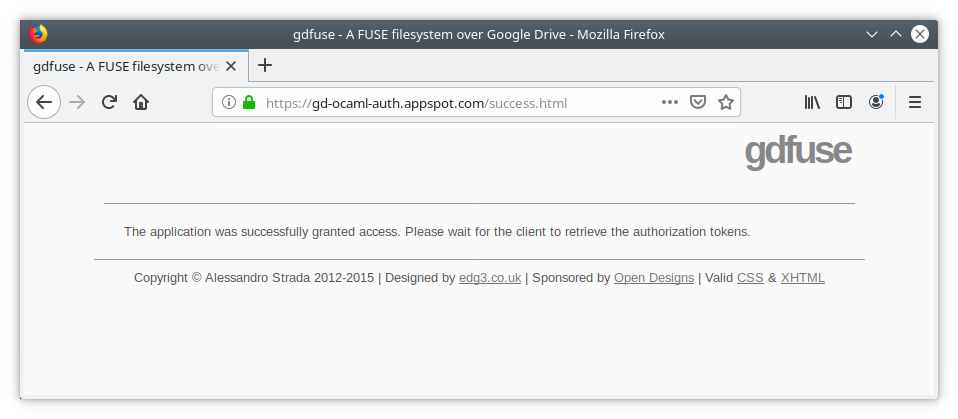
\includegraphics[scale=0.47]{images/ocaml7.png}
    \caption{Screenshot ocaml7.png}        % pmateti
    \label{fig:ocaml7}
  \end{figure}
\item Make Directory and Mount Drive
\begin{verbatim}
  hanen@hanen:mkdir ~/GoogleDrive
  hanen@hanen:google-drive-ocamlfuse ~/GoogleDrive
  hanen@hanen:cd GoogleDrive
  hanen@hanen:ls
  '2019-Hanen-CS 6970'    Misc
\end{verbatim}
That final output matches the contents of the Google Drive in the
browser as seen in Figure \ref{fig:ocaml10}
\begin{figure}[htb]
  \centering
  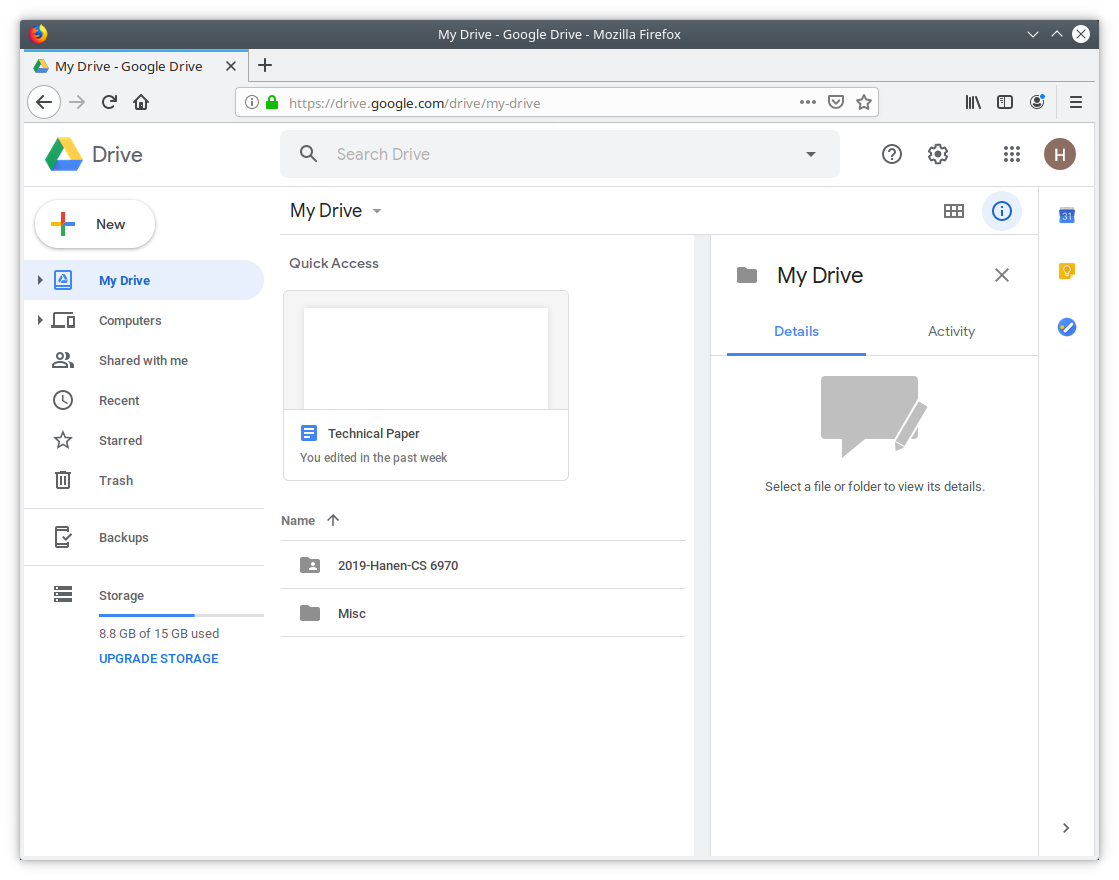
\includegraphics[scale=0.4]{images/ocaml10.png}
  \caption{Content of GD as seen through the browser} % pmateti
  \label{fig:ocaml10}
\end{figure}
\end{enumerate}
\subsection{Mount Google Drive on Android Tablet}
As a primary goal of this project, the next step is to have OCamlFUSE function similarly to the previous section using an Android device. Therefore, my attention turned to cross compilers in an effort to compile the OCaml code of OCamlFUSE into an executable that would be compatible with Android (ARM processor). I discovered several cross compilers and decided to try a few.
\subsubsection{OCaml-Cross}
Following the first compiler I found \cite{crosscompiler}, I did not manage to get very far before I ran into errors. The following are the commands I ran and their output:
\begin{verbatim}
hanen@hanen:~/Desktop/google-drive-ocamlfuse-beta$ sudo su
root@hanen:/home/hanen/Desktop/google-drive-ocamlfuse-beta# opam repository 
add android git://github.com/whitequark/opam-cross-android
[WARNING] Running as root is not recommended
[android] synchronised from git://github.com/whitequark/opam-cross-android
[WARNING] The repository 'android' at git://github.com/whitequark/opam-
cross-android doesn't have a 'repo'
          file, and might not be compatible with this version of opam.
[NOTE] Repository at git://github.com/whitequark/opam-cross-android 
doesn't define its version, assuming
       it's 1.2.

<><> Upgrading repositories from older opam format ><><><><><><><><>
Upgrading repository "android"...
[ERROR] Unconvertible 'available:' disjunction in
        /root/.opam/repo/android/packages/ocaml-android32.4.04.0/opam
[NOTE] Repository android has been added to the selections of switch 
default only.
       Run `opam repository add android --all-switches|--set-default' 
       to use it in all existing switches,
       or in newly created switches, respectively.

root@hanen:/home/hanen/Desktop/google-drive-ocamlfuse-beta# opam 
switch 4.04.0+32bit
[WARNING] Running as root is not recommended
[ERROR] No switch 4.04.0+32bit is currently installed. Did you 
mean 'opam switch create 4.04.0+32bit'?
        Installed switches are:
          - default

root@hanen:/home/hanen/Desktop/google-drive-ocamlfuse-beta# opam 
switch create 4.04.0+32bit
[WARNING] Running as root is not recommended

<><> Gathering sources ><><><><><><><><><><><><><><><><><><><><><>
[ocaml-variants.4.04.0+32bit] downloaded from cache at 
https://opam.ocaml.org/cache

<><> Processing actions <><><><><><><><><><><><><><><><><><><><><>
∗ installed base-bigarray.base
∗ installed base-threads.base
∗ installed base-unix.base
[ERROR] The compilation of ocaml-variants failed at 
"/root/.opam/opam-init/hooks/sandbox.sh build
        ./configure -prefix /root/.opam/4.04.0+32bit 
        -with-debug-runtime -cc gcc -m32 -as as --32 -aspp gcc
        -m32 -c -host i386-linux -partialld ld -r -melf_i386".

#=== ERROR while compiling ocaml-variants.4.04.0+32bit ==========#
# context     2.0.4 | linux/x86_64 |  | https://opam.ocaml.org#3389beb3
# path        ~/.opam/4.04.0+32bit/.opam-switch/build/ocaml-
variants.4.04.0+32bit
# command     ~/.opam/opam-init/hooks/sandbox.sh build ./configure -prefix 
/root/.opam/4.04.0+32bit -with-debug-runtime -cc gcc -m32 -as as --32 
-aspp gcc -m32 -c -host i386-linux -partialld ld -r -melf_i386
# exit-code   2
# env-file    ~/.opam/log/ocaml-variants-11817-ad8886.env
# output-file ~/.opam/log/ocaml-variants-11817-ad8886.out
### output ###
# Configuring OCaml version 4.04.0
# Configuring for host i386-pc-linux-gnu ...
# Configuring for target i386-pc-linux-gnu ...
# Using compiler gcc -m32.
# Compiler family and version: gcc-8-3.
# [ERROR!] Unable to compile the test program.
#  Make sure the C compiler gcc -m32  is properly installed.



<><> Error report <><><><><><><><><><><><><><><><><><><><><><><>
┌─ The following actions failed
│ λ build ocaml-variants 4.04.0+32bit
└─ 
┌─ The following changes have been performed (the rest was aborted)
│ ∗ install base-bigarray base
│ ∗ install base-threads  base
│ ∗ install base-unix     base
└─ 
# Run eval $(opam env) to update the current shell environment
Switch initialisation failed: clean up? ('n' will leave the 
switch partially installed) [Y/n] y
\end{verbatim}
Right away, there is an error reporting the inability to find the android repository and that the version of OPam being used may not be compatible. I try to ignore this and trudge forward with the switch command, but the response gives me a heads up that the switch I am attempting to use has not been created. The response is very helpful and gives me the exact command I need to execute in order to create the switch I'm trying to use. So, I execute this command only to find more errors. These are beyond the scope of my understanding of OPam and OCaml, so I unable to proceed. I Google for hours, but find no viable way around this. 
\subsubsection{OCaml-ARM}
My Googling leads me to another cross compiler that I decide to attempt \cite{armcompiler}. Again, I am faced with issues I must try to work around. This is not as simple as following the list of commands supplied on the GitHub page. The first few commands execute without any obstacles.
\begin{verbatim}
root@hanen:/home/hanen/Desktop/google-drive-ocamlfuse-beta# 
sudo dpkg --add-architecture armhf
root@hanen:/home/hanen/Desktop/google-drive-ocamlfuse-beta# 
sudo dpkg --add-architecture i386
root@hanen:/home/hanen/Desktop/google-drive-ocamlfuse-beta# 
sudo apt-get update
Hit:1 http://security.ubuntu.com/ubuntu cosmic-security 
InRelease
Hit:2 http://packages.microsoft.com/repos/vscode stable 
InRelease                                          
Ign:3 http://packages.cloud.google.com/apt gcsfuse-cosmic 
InRelease                                        
Hit:4 http://ppa.launchpad.net/alessandro-strada/ppa/ubuntu 
cosmic InRelease                               
Hit:5 http://us.archive.ubuntu.com/ubuntu cosmic InRelease                                                 
Err:6 http://packages.cloud.google.com/apt gcsfuse-cosmic 
Release                                          
  404  Not Found [IP: 172.217.12.46 80]
Hit:7 http://apt.insynchq.com/ubuntu cosmic InRelease                                                      
Hit:8 http://us.archive.ubuntu.com/ubuntu cosmic-updates 
InRelease                                         
Hit:9 http://us.archive.ubuntu.com/ubuntu cosmic-backports 
InRelease                                       
Ign:10 http://security.ubuntu.com/ubuntu 
cosmic-security/main armhf Packages                               
Ign:11 http://security.ubuntu.com/ubuntu 
cosmic-security/restricted armhf Packages
Ign:12 http://security.ubuntu.com/ubuntu 
cosmic-security/universe armhf Packages
Ign:13 http://security.ubuntu.com/ubuntu 
cosmic-security/multiverse armhf Packages
Hit:14 http://ppa.launchpad.net/avsm/ppa/ubuntu 
cosmic InRelease         
Ign:10 http://security.ubuntu.com/ubuntu 
cosmic-security/main armhf Packages
Ign:11 http://security.ubuntu.com/ubuntu 
cosmic-security/restricted armhf Packages
Ign:12 http://security.ubuntu.com/ubuntu 
cosmic-security/universe armhf Packages
Ign:13 http://security.ubuntu.com/ubuntu 
cosmic-security/multiverse armhf Packages
Ign:10 http://security.ubuntu.com/ubuntu 
cosmic-security/main armhf Packages
Ign:11 http://security.ubuntu.com/ubuntu 
cosmic-security/restricted armhf Packages
Ign:12 http://security.ubuntu.com/ubuntu 
cosmic-security/universe armhf Packages
Ign:13 http://security.ubuntu.com/ubuntu 
cosmic-security/multiverse armhf Packages
Ign:10 http://security.ubuntu.com/ubuntu 
cosmic-security/main armhf Packages
Ign:11 http://security.ubuntu.com/ubuntu 
cosmic-security/restricted armhf Packages
Ign:12 http://security.ubuntu.com/ubuntu 
cosmic-security/universe armhf Packages
Ign:13 http://security.ubuntu.com/ubuntu 
cosmic-security/multiverse armhf Packages
Ign:10 http://security.ubuntu.com/ubuntu 
cosmic-security/main armhf Packages
Ign:11 http://security.ubuntu.com/ubuntu 
cosmic-security/restricted armhf Packages
Ign:12 http://security.ubuntu.com/ubuntu 
cosmic-security/universe armhf Packages
Ign:13 http://security.ubuntu.com/ubuntu 
cosmic-security/multiverse armhf Packages
Err:10 http://security.ubuntu.com/ubuntu 
cosmic-security/main armhf Packages
  404  Not Found [IP: 91.189.91.23 80]
Ign:11 http://security.ubuntu.com/ubuntu 
cosmic-security/restricted armhf Packages
Ign:15 http://us.archive.ubuntu.com/ubuntu 
cosmic/main armhf Packages
Ign:12 http://security.ubuntu.com/ubuntu 
cosmic-security/universe armhf Packages
Ign:13 http://security.ubuntu.com/ubuntu 
cosmic-security/multiverse armhf Packages
Ign:16 http://us.archive.ubuntu.com/ubuntu 
cosmic/restricted armhf Packages
Ign:17 http://us.archive.ubuntu.com/ubuntu 
cosmic/universe armhf Packages
Ign:18 http://us.archive.ubuntu.com/ubuntu 
cosmic/multiverse armhf Packages
Ign:15 http://us.archive.ubuntu.com/ubuntu 
cosmic/main armhf Packages
Ign:16 http://us.archive.ubuntu.com/ubuntu 
cosmic/restricted armhf Packages
Ign:17 http://us.archive.ubuntu.com/ubuntu 
cosmic/universe armhf Packages
Ign:18 http://us.archive.ubuntu.com/ubuntu 
cosmic/multiverse armhf Packages
Ign:15 http://us.archive.ubuntu.com/ubuntu 
cosmic/main armhf Packages
Ign:16 http://us.archive.ubuntu.com/ubuntu 
cosmic/restricted armhf Packages
Ign:17 http://us.archive.ubuntu.com/ubuntu 
cosmic/universe armhf Packages
Ign:18 http://us.archive.ubuntu.com/ubuntu 
cosmic/multiverse armhf Packages
Ign:15 http://us.archive.ubuntu.com/ubuntu 
cosmic/main armhf Packages
Ign:16 http://us.archive.ubuntu.com/ubuntu 
cosmic/restricted armhf Packages
Ign:17 http://us.archive.ubuntu.com/ubuntu 
cosmic/universe armhf Packages
Ign:18 http://us.archive.ubuntu.com/ubuntu 
cosmic/multiverse armhf Packages
Ign:15 http://us.archive.ubuntu.com/ubuntu 
cosmic/main armhf Packages
Ign:19 http://us.archive.ubuntu.com/ubuntu 
cosmic-updates/main armhf Packages
Ign:20 http://us.archive.ubuntu.com/ubuntu 
cosmic-updates/restricted armhf Packages
Ign:21 http://us.archive.ubuntu.com/ubuntu 
cosmic-updates/universe armhf Packages
Ign:22 http://us.archive.ubuntu.com/ubuntu 
cosmic-updates/multiverse armhf Packages
Ign:16 http://us.archive.ubuntu.com/ubuntu 
cosmic/restricted armhf Packages
Ign:17 http://us.archive.ubuntu.com/ubuntu 
cosmic/universe armhf Packages
Ign:18 http://us.archive.ubuntu.com/ubuntu 
cosmic/multiverse armhf Packages
Err:15 http://us.archive.ubuntu.com/ubuntu 
cosmic/main armhf Packages
  404  Not Found [IP: 91.189.91.23 80]
Ign:19 http://us.archive.ubuntu.com/ubuntu 
cosmic-updates/main armhf Packages
Ign:20 http://us.archive.ubuntu.com/ubuntu 
cosmic-updates/restricted armhf Packages
Ign:21 http://us.archive.ubuntu.com/ubuntu 
cosmic-updates/universe armhf Packages
Ign:22 http://us.archive.ubuntu.com/ubuntu 
cosmic-updates/multiverse armhf Packages
Ign:16 http://us.archive.ubuntu.com/ubuntu 
cosmic/restricted armhf Packages
Ign:17 http://us.archive.ubuntu.com/ubuntu 
cosmic/universe armhf Packages
Ign:18 http://us.archive.ubuntu.com/ubuntu 
cosmic/multiverse armhf Packages
Ign:19 http://us.archive.ubuntu.com/ubuntu 
cosmic-updates/main armhf Packages
Ign:20 http://us.archive.ubuntu.com/ubuntu 
cosmic-updates/restricted armhf Packages
Ign:21 http://us.archive.ubuntu.com/ubuntu 
cosmic-updates/universe armhf Packages
Ign:22 http://us.archive.ubuntu.com/ubuntu 
cosmic-updates/multiverse armhf Packages
Ign:23 http://us.archive.ubuntu.com/ubuntu 
cosmic-backports/main armhf Packages
Ign:24 http://us.archive.ubuntu.com/ubuntu 
cosmic-backports/universe armhf Packages
Ign:19 http://us.archive.ubuntu.com/ubuntu 
cosmic-updates/main armhf Packages
Ign:20 http://us.archive.ubuntu.com/ubuntu 
cosmic-updates/restricted armhf Packages
Ign:21 http://us.archive.ubuntu.com/ubuntu 
cosmic-updates/universe armhf Packages
Ign:22 http://us.archive.ubuntu.com/ubuntu 
cosmic-updates/multiverse armhf Packages
Ign:23 http://us.archive.ubuntu.com/ubuntu 
cosmic-backports/main armhf Packages
Ign:24 http://us.archive.ubuntu.com/ubuntu 
cosmic-backports/universe armhf Packages
Ign:19 http://us.archive.ubuntu.com/ubuntu 
cosmic-updates/main armhf Packages
Ign:20 http://us.archive.ubuntu.com/ubuntu 
cosmic-updates/restricted armhf Packages
Ign:21 http://us.archive.ubuntu.com/ubuntu 
cosmic-updates/universe armhf Packages
Ign:22 http://us.archive.ubuntu.com/ubuntu 
cosmic-updates/multiverse armhf Packages
Ign:23 http://us.archive.ubuntu.com/ubuntu 
cosmic-backports/main armhf Packages
Ign:24 http://us.archive.ubuntu.com/ubuntu 
cosmic-backports/universe armhf Packages
Err:19 http://us.archive.ubuntu.com/ubuntu 
cosmic-updates/main armhf Packages
  404  Not Found [IP: 91.189.91.23 80]
Ign:20 http://us.archive.ubuntu.com/ubuntu 
cosmic-updates/restricted armhf Packages
Ign:21 http://us.archive.ubuntu.com/ubuntu 
cosmic-updates/universe armhf Packages
Ign:22 http://us.archive.ubuntu.com/ubuntu 
cosmic-updates/multiverse armhf Packages
Ign:23 http://us.archive.ubuntu.com/ubuntu 
cosmic-backports/main armhf Packages
Ign:24 http://us.archive.ubuntu.com/ubuntu 
cosmic-backports/universe armhf Packages
Ign:23 http://us.archive.ubuntu.com/ubuntu 
cosmic-backports/main armhf Packages
Ign:24 http://us.archive.ubuntu.com/ubuntu 
cosmic-backports/universe armhf Packages
Err:23 http://us.archive.ubuntu.com/ubuntu 
cosmic-backports/main armhf Packages
  404  Not Found [IP: 91.189.91.23 80]
Ign:24 http://us.archive.ubuntu.com/ubuntu 
cosmic-backports/universe armhf Packages
Reading package lists... Done
E: The repository 'http://packages.cloud.google.com/apt 
gcsfuse-cosmic Release' does not have a Release file.
N: Updating from such a repository can't be done 
securely, and is therefore disabled by default.
N: See apt-secure(8) manpage for repository 
creation and user configuration details.
N: Skipping acquire of configured file 
'non-free/binary-armhf/Packages' as repository 
'http://apt.insynchq.com/ubuntu cosmic InRelease' 
doesn't support architecture 'armhf'
N: Skipping acquire of configured file 
'contrib/binary-armhf/Packages' as repository 
'http://apt.insynchq.com/ubuntu cosmic InRelease' 
doesn't support architecture 'armhf'
root@hanen:/home/hanen/Desktop/google-drive-ocamlfuse-beta# 
sudo apt-get install gcc-4.9-arm-linux-gnueabihf 
gcc-arm-linux-gnueabihf libc6-dev:armhf libgcc-4.9-dev:armhf 
linux-libc-dev:i386 opam
Reading package lists... Done
Building dependency tree       
Reading state information... Done
Package gcc-4.9-arm-linux-gnueabihf is not available, 
but is referred to by another package.
This may mean that the package is missing, has been 
obsoleted, or is only available from another source

E: Package 'gcc-4.9-arm-linux-gnueabihf' has no 
installation candidate
E: Unable to locate package libc6-dev:armhf
E: Unable to locate package libgcc-4.9-dev:armhf
E: Couldn't find any package by glob 'libgcc-4.9-dev'
E: Couldn't find any package by regex 'libgcc-4.9-dev'
\end{verbatim}
This is where the problems crop up. I have seen this many times throughout the span of working on this project; this issue of not being able to locate certain packages. I, unfortunately, have not pinpointed a solution for this particular bump in the road. In this particular case, I decide to take the last command, \verb|sudo apt-get install| \verb| gcc-4.9-arm-linux-gnueabihf| \verb| gcc-arm-linux-gnueabihf| \verb| libc6-dev:armhf|\\ \verb| libgcc-4.9-dev:armhf| \verb| linux-libc-dev:i386 opam|, and break it up into multiple \verb|apt-get install| executions so that I can try to isolate the package that is causing the problem.
\begin{verbatim}
root@hanen:/home/hanen/Desktop/google-drive-ocamlfuse-beta# 
sudo apt-get install gcc-4.9-arm-linux-gnueabihfReading 
package lists... Done
Building dependency tree       
Reading state information... Done
Package gcc-4.9-arm-linux-gnueabihf is not available, 
but is referred to by another package.
This may mean that the package is missing, has been 
obsoleted, or
is only available from another source

E: Package 'gcc-4.9-arm-linux-gnueabihf' has no 
installation candidate
root@hanen:/home/hanen/Desktop/google-drive-ocamlfuse-beta# 
sudo apt-get install gcc-arm-linux-gnueabihf    Reading 
package lists... Done
Building dependency tree       
Reading state information... Done
The following packages were automatically installed and are 
no longer required:
  libncursesw5 libtinfo5
Use 'sudo apt autoremove' to remove them.
The following additional packages will be installed:
  binutils-arm-linux-gnueabihf cpp-8-arm-linux-gnueabihf 
  cpp-arm-linux-gnueabihf gcc-8-arm-linux-gnueabihf
  gcc-8-arm-linux-gnueabihf-base gcc-8-cross-base 
  libasan5-armhf-cross libatomic1-armhf-cross
  libc6-armhf-cross libc6-dev-armhf-cross 
  libgcc-8-dev-armhf-cross libgcc1-armhf-cross
  libgomp1-armhf-cross libstdc++6-armhf-cross 
  libubsan1-armhf-cross linux-libc-dev-armhf-cross
Suggested packages:
  binutils-doc gcc-8-locales cpp-doc 
  gcc-8-multilib-arm-linux-gnueabihf gcc-8-doc 
  libgcc1-dbg-armhf-cross
  libgomp1-dbg-armhf-cross libitm1-dbg-armhf-cross 
  libatomic1-dbg-armhf-cross libasan5-dbg-armhf-cross
  liblsan0-dbg-armhf-cross libtsan0-dbg-armhf-cross 
  libubsan1-dbg-armhf-cross libmpx2-dbg-armhf-cross
  libquadmath0-dbg-armhf-cross autoconf automake 
  libtool flex bison gdb-arm-linux-gnueabihf gcc-doc
The following NEW packages will be installed:
  binutils-arm-linux-gnueabihf cpp-8-arm-linux-gnueabihf 
  cpp-arm-linux-gnueabihf gcc-8-arm-linux-gnueabihf
  gcc-8-arm-linux-gnueabihf-base gcc-8-cross-base 
  gcc-arm-linux-gnueabihf libasan5-armhf-cross
  libatomic1-armhf-cross libc6-armhf-cross 
  libc6-dev-armhf-cross libgcc-8-dev-armhf-cross
  libgcc1-armhf-cross libgomp1-armhf-cross 
  libstdc++6-armhf-cross libubsan1-armhf-cross
  linux-libc-dev-armhf-cross
0 upgraded, 17 newly installed, 0 to remove and 10 not 
upgraded.
Need to get 22.3 MB of archives.
After this operation, 72.8 MB of additional disk space 
will be used.
Do you want to continue? [Y/n] y
Get:1 http://us.archive.ubuntu.com/ubuntu 
cosmic-updates/main amd64 gcc-8-arm-linux-gnueabihf-base 
amd64 8.3.0-6ubuntu1~18.10.1cross1 [19.0 kB]
Get:2 http://us.archive.ubuntu.com/ubuntu 
cosmic-updates/main amd64 cpp-8-arm-linux-gnueabihf 
amd64 8.3.0-6ubuntu1~18.10.1cross1 [6,634 kB]
Get:3 http://us.archive.ubuntu.com/ubuntu 
cosmic-updates/main amd64 cpp-arm-linux-gnueabihf 
amd64 4:8.3.0-1ubuntu1.2 [3,520 B]
Get:4 http://us.archive.ubuntu.com/ubuntu 
cosmic-updates/main amd64 binutils-arm-linux-gnueabihf 
amd64 2.31.1-6ubuntu1.2 [2,799 kB]
Get:5 http://us.archive.ubuntu.com/ubuntu 
cosmic-updates/main amd64 gcc-8-cross-base all 
8.3.0-6ubuntu1~18.10.1cross1 [13.7 kB]
Get:6 http://us.archive.ubuntu.com/ubuntu 
cosmic/main amd64 libc6-armhf-cross all 
2.28-0ubuntu1cross1 [967 kB]
Get:7 http://us.archive.ubuntu.com/ubuntu 
cosmic-updates/main amd64 libgcc1-armhf-cross all 
1:8.3.0-6ubuntu1~18.10.1cross1 [37.2 kB]
Get:8 http://us.archive.ubuntu.com/ubuntu 
cosmic-updates/main amd64 libgomp1-armhf-cross all 
8.3.0-6ubuntu1~18.10.1cross1 [65.1 kB]
Get:9 http://us.archive.ubuntu.com/ubuntu 
cosmic-updates/main amd64 libatomic1-armhf-cross all 
8.3.0-6ubuntu1~18.10.1cross1 [6,896 B]
Get:10 http://us.archive.ubuntu.com/ubuntu 
cosmic-updates/main amd64 libasan5-armhf-cross all 
8.3.0-6ubuntu1~18.10.1cross1 [341 kB]
Get:11 http://us.archive.ubuntu.com/ubuntu 
cosmic-updates/main amd64 libstdc++6-armhf-cross all 
8.3.0-6ubuntu1~18.10.1cross1 [312 kB]
Get:12 http://us.archive.ubuntu.com/ubuntu 
cosmic-updates/main amd64 libubsan1-armhf-cross all 
8.3.0-6ubuntu1~18.10.1cross1 [107 kB]
Get:13 http://us.archive.ubuntu.com/ubuntu 
cosmic-updates/main amd64 libgcc-8-dev-armhf-cross all 
8.3.0-6ubuntu1~18.10.1cross1 [631 kB]
Get:14 http://us.archive.ubuntu.com/ubuntu 
cosmic-updates/main amd64 gcc-8-arm-linux-gnueabihf amd64 
8.3.0-6ubuntu1~18.10.1cross1 [7,395 kB]
Get:15 http://us.archive.ubuntu.com/ubuntu 
cosmic-updates/main amd64 gcc-arm-linux-gnueabihf amd64 
4:8.3.0-1ubuntu1.2 [1,428 B]
Get:16 http://us.archive.ubuntu.com/ubuntu cosmic/main amd64 
linux-libc-dev-armhf-cross all 4.18.0-8.9cross1 [981 kB]
Get:17 http://us.archive.ubuntu.com/ubuntu cosmic/main amd64 
libc6-dev-armhf-cross all 2.28-0ubuntu1cross1 [1,945 kB]
Fetched 22.3 MB in 6s (3,517 kB/s)                                                                         
Selecting previously unselected package gcc-8-arm-linux-
gnueabihf-base:amd64.
(Reading database ... 245405 files and directories currently 
installed.)
Preparing to unpack .../00-gcc-8-arm-linux-gnueabihf-
base_8.3.0-6ubuntu1~18.10.1cross1_amd64.deb ...
Unpacking gcc-8-arm-linux-gnueabihf-base:amd64 (8.3.0-6ubuntu1~
18.10.1cross1) ...
Selecting previously unselected package cpp-8-arm-linux-gnueabihf.
Preparing to unpack .../01-cpp-8-arm-linux-gnueabihf_8.3.0-6ubuntu1~
18.10.1cross1_amd64.deb ...
Unpacking cpp-8-arm-linux-gnueabihf (8.3.0-6ubuntu1~18.10.1cross1) ...
Selecting previously unselected package cpp-arm-linux-gnueabihf.
Preparing to unpack .../02-cpp-arm-linux-gnueabihf_4%3a8.3.0-
1ubuntu1.2_amd64.deb ...
Unpacking cpp-arm-linux-gnueabihf (4:8.3.0-1ubuntu1.2) ...
Selecting previously unselected package binutils-arm-linux-gnueabihf.
Preparing to unpack .../03-binutils-arm-linux-gnueabihf_2.31.1-
6ubuntu1.2_amd64.deb ...
Unpacking binutils-arm-linux-gnueabihf (2.31.1-6ubuntu1.2) ...
Selecting previously unselected package gcc-8-cross-base.
Preparing to unpack .../04-gcc-8-cross-base_8.3.0-6ubuntu1~
18.10.1cross1_all.deb ...
Unpacking gcc-8-cross-base (8.3.0-6ubuntu1~18.10.1cross1) ...
Selecting previously unselected package libc6-armhf-cross.
Preparing to unpack .../05-libc6-armhf-cross_2.28-
0ubuntu1cross1_all.deb ...
Unpacking libc6-armhf-cross (2.28-0ubuntu1cross1) ...
Selecting previously unselected package libgcc1-armhf-cross.
Preparing to unpack .../06-libgcc1-armhf-cross_1%3a8.3.0-6ubuntu1~
18.10.1cross1_all.deb ...
Unpacking libgcc1-armhf-cross (1:8.3.0-6ubuntu1~18.10.1cross1) ...
Selecting previously unselected package libgomp1-armhf-cross.
Preparing to unpack .../07-libgomp1-armhf-cross_8.3.0-6ubuntu1~
18.10.1cross1_all.deb ...
Unpacking libgomp1-armhf-cross (8.3.0-6ubuntu1~18.10.1cross1) ...
Selecting previously unselected package libatomic1-armhf-cross.
Preparing to unpack .../08-libatomic1-armhf-cross_8.3.0-6ubuntu1~
18.10.1cross1_all.deb ...
Unpacking libatomic1-armhf-cross (8.3.0-6ubuntu1~18.10.1cross1) ...
Selecting previously unselected package libasan5-armhf-cross.
Preparing to unpack .../09-libasan5-armhf-cross_8.3.0-6ubuntu1~
18.10.1cross1_all.deb ...
Unpacking libasan5-armhf-cross (8.3.0-6ubuntu1~18.10.1cross1) ...
Selecting previously unselected package libstdc++6-armhf-cross.
Preparing to unpack .../10-libstdc++6-armhf-cross_8.3.0-6ubuntu1~
18.10.1cross1_all.deb ...
Unpacking libstdc++6-armhf-cross (8.3.0-6ubuntu1~18.10.1cross1) ...
Selecting previously unselected package libubsan1-armhf-cross.
Preparing to unpack .../11-libubsan1-armhf-cross_8.3.0-6ubuntu1~
18.10.1cross1_all.deb ...
Unpacking libubsan1-armhf-cross (8.3.0-6ubuntu1~18.10.1cross1) ...
Selecting previously unselected package libgcc-8-dev-armhf-cross.
Preparing to unpack .../12-libgcc-8-dev-armhf-cross_8.3.0-6ubuntu1~
18.10.1cross1_all.deb ...
Unpacking libgcc-8-dev-armhf-cross (8.3.0-6ubuntu1~18.10.1cross1) ...
Selecting previously unselected package gcc-8-arm-linux-gnueabihf.
Preparing to unpack .../13-gcc-8-arm-linux-gnueabihf_8.3.0-6ubuntu1~
18.10.1cross1_amd64.deb ...
Unpacking gcc-8-arm-linux-gnueabihf (8.3.0-6ubuntu1~18.10.1cross1) ...
Selecting previously unselected package gcc-arm-linux-gnueabihf.
Preparing to unpack .../14-gcc-arm-linux-gnueabihf_4%3a8.3.0-
1ubuntu1.2_amd64.deb ...
Unpacking gcc-arm-linux-gnueabihf (4:8.3.0-1ubuntu1.2) ...
Selecting previously unselected package linux-libc-dev-armhf-cross.
Preparing to unpack .../15-linux-libc-dev-armhf-cross_4.18.0-
8.9cross1_all.deb ...
Unpacking linux-libc-dev-armhf-cross (4.18.0-8.9cross1) ...
Selecting previously unselected package libc6-dev-armhf-cross.
Preparing to unpack .../16-libc6-dev-armhf-cross_2.28-
0ubuntu1cross1_all.deb ...
Unpacking libc6-dev-armhf-cross (2.28-0ubuntu1cross1) ...
Setting up gcc-8-cross-base (8.3.0-6ubuntu1~18.10.1cross1) ...
Setting up libc6-armhf-cross (2.28-0ubuntu1cross1) ...
Setting up libgcc1-armhf-cross (1:8.3.0-6ubuntu1~18.10.1cross1) ...
Setting up libstdc++6-armhf-cross (8.3.0-6ubuntu1~18.10.1cross1) ...
Setting up libubsan1-armhf-cross (8.3.0-6ubuntu1~18.10.1cross1) ...
Setting up binutils-arm-linux-gnueabihf (2.31.1-6ubuntu1.2) ...
Setting up libgomp1-armhf-cross (8.3.0-6ubuntu1~18.10.1cross1) ...
Setting up linux-libc-dev-armhf-cross (4.18.0-8.9cross1) ...
Setting up libatomic1-armhf-cross (8.3.0-6ubuntu1~18.10.1cross1) ...
Processing triggers for libc-bin (2.28-0ubuntu1) ...
Processing triggers for man-db (2.8.4-2) ...
Setting up gcc-8-arm-linux-gnueabihf-base:amd64 (8.3.0-6ubuntu1~
18.10.1cross1) ...
Setting up libasan5-armhf-cross (8.3.0-6ubuntu1~18.10.1cross1) ...
Setting up libgcc-8-dev-armhf-cross (8.3.0-6ubuntu1~18.10.1cross1) ...
Setting up libc6-dev-armhf-cross (2.28-0ubuntu1cross1) ...
Setting up cpp-8-arm-linux-gnueabihf (8.3.0-6ubuntu1~18.10.1cross1) ...
Setting up cpp-arm-linux-gnueabihf (4:8.3.0-1ubuntu1.2) ...
Setting up gcc-8-arm-linux-gnueabihf (8.3.0-6ubuntu1~18.10.1cross1) ...
Setting up gcc-arm-linux-gnueabihf (4:8.3.0-1ubuntu1.2) ...
root@hanen:/home/hanen/Desktop/google-drive-ocamlfuse-beta# 
sudo apt-get install libc6-dev:armhf
Reading package lists... Done
Building dependency tree       
Reading state information... Done
E: Unable to locate package libc6-dev:armhf
root@hanen:/home/hanen/Desktop/google-drive-ocamlfuse-beta# 
sudo apt-get install libgcc-4.9-dev:armhf
Reading package lists... Done
Building dependency tree       
Reading state information... Done
E: Unable to locate package libgcc-4.9-dev:armhf
E: Couldn't find any package by glob 'libgcc-4.9-dev'
E: Couldn't find any package by regex 'libgcc-4.9-dev'
root@hanen:/home/hanen/Desktop/google-drive-ocamlfuse-beta# 
sudo apt-get install linux-libc-dev:i386 
Reading package lists... Done
Building dependency tree       
Reading state information... Done
The following packages were automatically installed and are no longer required:
  libncursesw5 libtinfo5
Use 'sudo apt autoremove' to remove them.
The following NEW packages will be installed:
  linux-libc-dev:i386
0 upgraded, 1 newly installed, 0 to remove and 10 not upgraded.
Need to get 1,009 kB of archives.
After this operation, 5,377 kB of additional disk space will be used.
Get:1 http://us.archive.ubuntu.com/ubuntu cosmic-updates/main i386 
linux-libc-dev i386 4.18.0-25.26 [1,009 kB]
Fetched 1,009 kB in 1s (1,083 kB/s)           
Selecting previously unselected package linux-libc-dev:i386.
(Reading database ... 247258 files and directories currently installed.)
Preparing to unpack .../linux-libc-dev_4.18.0-25.26_i386.deb ...
Unpacking linux-libc-dev:i386 (4.18.0-25.26) ...
Setting up linux-libc-dev:i386 (4.18.0-25.26) ...
\end{verbatim}
I have found success in installing \verb|gcc-arm-linux-gnueabihf| and \verb|linux-libc-dev:i386|, but I am blocked when trying to install \verb|gcc-4.9-arm-linux-gnueabihf|, \verb|libc6-dev:armhf|, and \verb|libgcc-4.9-dev:armhf|. Multiple attempts are not enough to install these packages so that this step is complete. Due to time limitation, I try to press forward and run the other commands to follow.
\begin{verbatim}
root@hanen:/home/hanen/Desktop/google-drive-ocamlfuse-beta# opam init
[WARNING] Running as root is not recommended

<><> Required setup - please read <><><><><><><><><><><><><><><><><><>

  In normal operation, opam only alters files within ~/.opam.

  However, to best integrate with your system, some environment variables
  should be set. If you allow it to, this initialisation step will update
  your bash configuration by adding the following line to ~/.profile:

    test -r /root/.opam/opam-init/init.sh && . /root/.opam/opam-init/init.sh >
    /dev/null 2> /dev/null || true

  Otherwise, every time you want to access your opam installation, you will
  need to run:

    eval $(opam env)

  You can always re-run this setup with 'opam init' later.

Do you want opam to modify ~/.profile? [N/y/f]
(default is 'no', use 'f' to choose a different file) y
A hook can be added to opam's init scripts to ensure that the shell remains 
in sync with the opam
environment when they are loaded. Set that up? [y/N] y

User configuration:
  ~/.profile is already up-to-date.
[NOTE] Make sure that ~/.profile is well sourced in your ~/.bashrc.

root@hanen:/home/hanen/Desktop/google-drive-ocamlfuse-beta# opam switch 4.02.1
[WARNING] Running as root is not recommended
[ERROR] No switch 4.02.1 is currently installed. Did you mean 'opam switch 
create 4.02.1'?
        Installed switches are:
          - 4.04.0
          - default

root@hanen:/home/hanen/Desktop/google-drive-ocamlfuse-beta# opam switch 
create 4.02.1
[WARNING] Running as root is not recommended

<><> Gathering sources ><><><><><><><><><><><><><><><><><><><><><><><>
[ocaml-base-compiler.4.02.1] downloaded from cache at 
https://opam.ocaml.org/cache

<><> Processing actions <><><><><><><><><><><><><><><><><><><><><><><>
∗ installed base-bigarray.base
∗ installed base-threads.base
∗ installed base-unix.base
∗ installed ocaml-base-compiler.4.02.1
∗ installed ocaml-config.1
∗ installed ocaml.4.02.1
∗ installed base-ocamlbuild.base
Done.
# Run eval $(opam env) to update the current shell environment
root@hanen:/home/hanen/Desktop/google-drive-ocamlfuse-beta# eval 
$(opam env)
[WARNING] Running as root is not recommended
root@hanen:/home/hanen/Desktop/google-drive-ocamlfuse-beta# opam 
install ocaml-src
[WARNING] Running as root is not recommended
The following actions will be performed:
  ∗ install ocaml-src 4.02.1

<><> Gathering sources ><><><><><><><><><><><><><><><><><><><><><><><>
[ocaml-src.4.02.1] found in cache

<><> Processing actions <><><><><><><><><><><><><><><><><><><><><><><>
∗ installed ocaml-src.4.02.1
Done.
root@hanen:/home/hanen/Desktop/google-drive-ocamlfuse-beta# git clone 
https://github.com/whirm/ocaml-arm
Cloning into 'ocaml-arm'...
remote: Enumerating objects: 183, done.
remote: Total 183 (delta 0), reused 0 (delta 0), pack-reused 183
Receiving objects: 100% (183/183), 29.74 KiB | 692.00 KiB/s, done.
Resolving deltas: 100% (84/84), done.
root@hanen:/home/hanen/Desktop/google-drive-ocamlfuse-beta# cd ocaml-arm
root@hanen:/home/hanen/Desktop/google-drive-ocamlfuse-beta/ocaml-arm# make
[WARNING] Running as root is not recommended
cp -a /root/.opam/4.02.1/lib/ocaml-src ocaml-src
touch stamp-copy
cd ocaml-src && \
./configure -prefix /root/.opam/4.02.1/arm-linux-gnueabihf \
        -bindir /root/.opam/4.02.1/bin/arm-linux-gnueabihf \
        -mandir /home/hanen/Desktop/google-drive-ocamlfuse-
        beta/ocaml-arm/no-man \
        -cc "gcc -m32" -as "gcc -m32 -c" -aspp "gcc -m32 -c" \
        -no-pthread
Configuring for host x86_64-unknown-linux-gnu ...
Configuring for target x86_64-unknown-linux-gnu ...
Using compiler gcc -m32.
[ERROR!]Unable to compile the test program.
 Make sure the C compiler gcc -m32 -O  is properly installed.
make: *** [Makefile:132: stamp-configure] Error 2
\end{verbatim}
The process seemed to be moving along well for the first few commands. However, I again ran into errors when trying to execute \verb|make|. I am not certain if my compiler is setup incorrectly or if previous failing steps may have led to this failure. At this point, I must declare defeat with regards to cross compiling OCamlFUSE in order to execute the application on an Android device. 